\section{Practice: Blinking LED Advanced}\label{pract:blinkingLEDAdvanced}

It will be very boring to just have a blinking LED. That is because in this practice we will be incorporating some hardware and software tweaks that will allow us to have a little more control over the LED. Or let's say, we will make a basic lamp.

What we want to prototype is a LED that turns on or off whenever we press a bottom. Before we dwell into detail, let's review what we will need:

\begin{itemize}
	\item A breadboard (we will be using Figure~\ref{fig:breadboard} as a guide).
	\item Wire to tie together the different parts of your circuit.
	\item One $10$K Ohm resistor.
	\item One pushbutton switch.	
\end{itemize}

\begin{figure}[htbp]
  \centering
  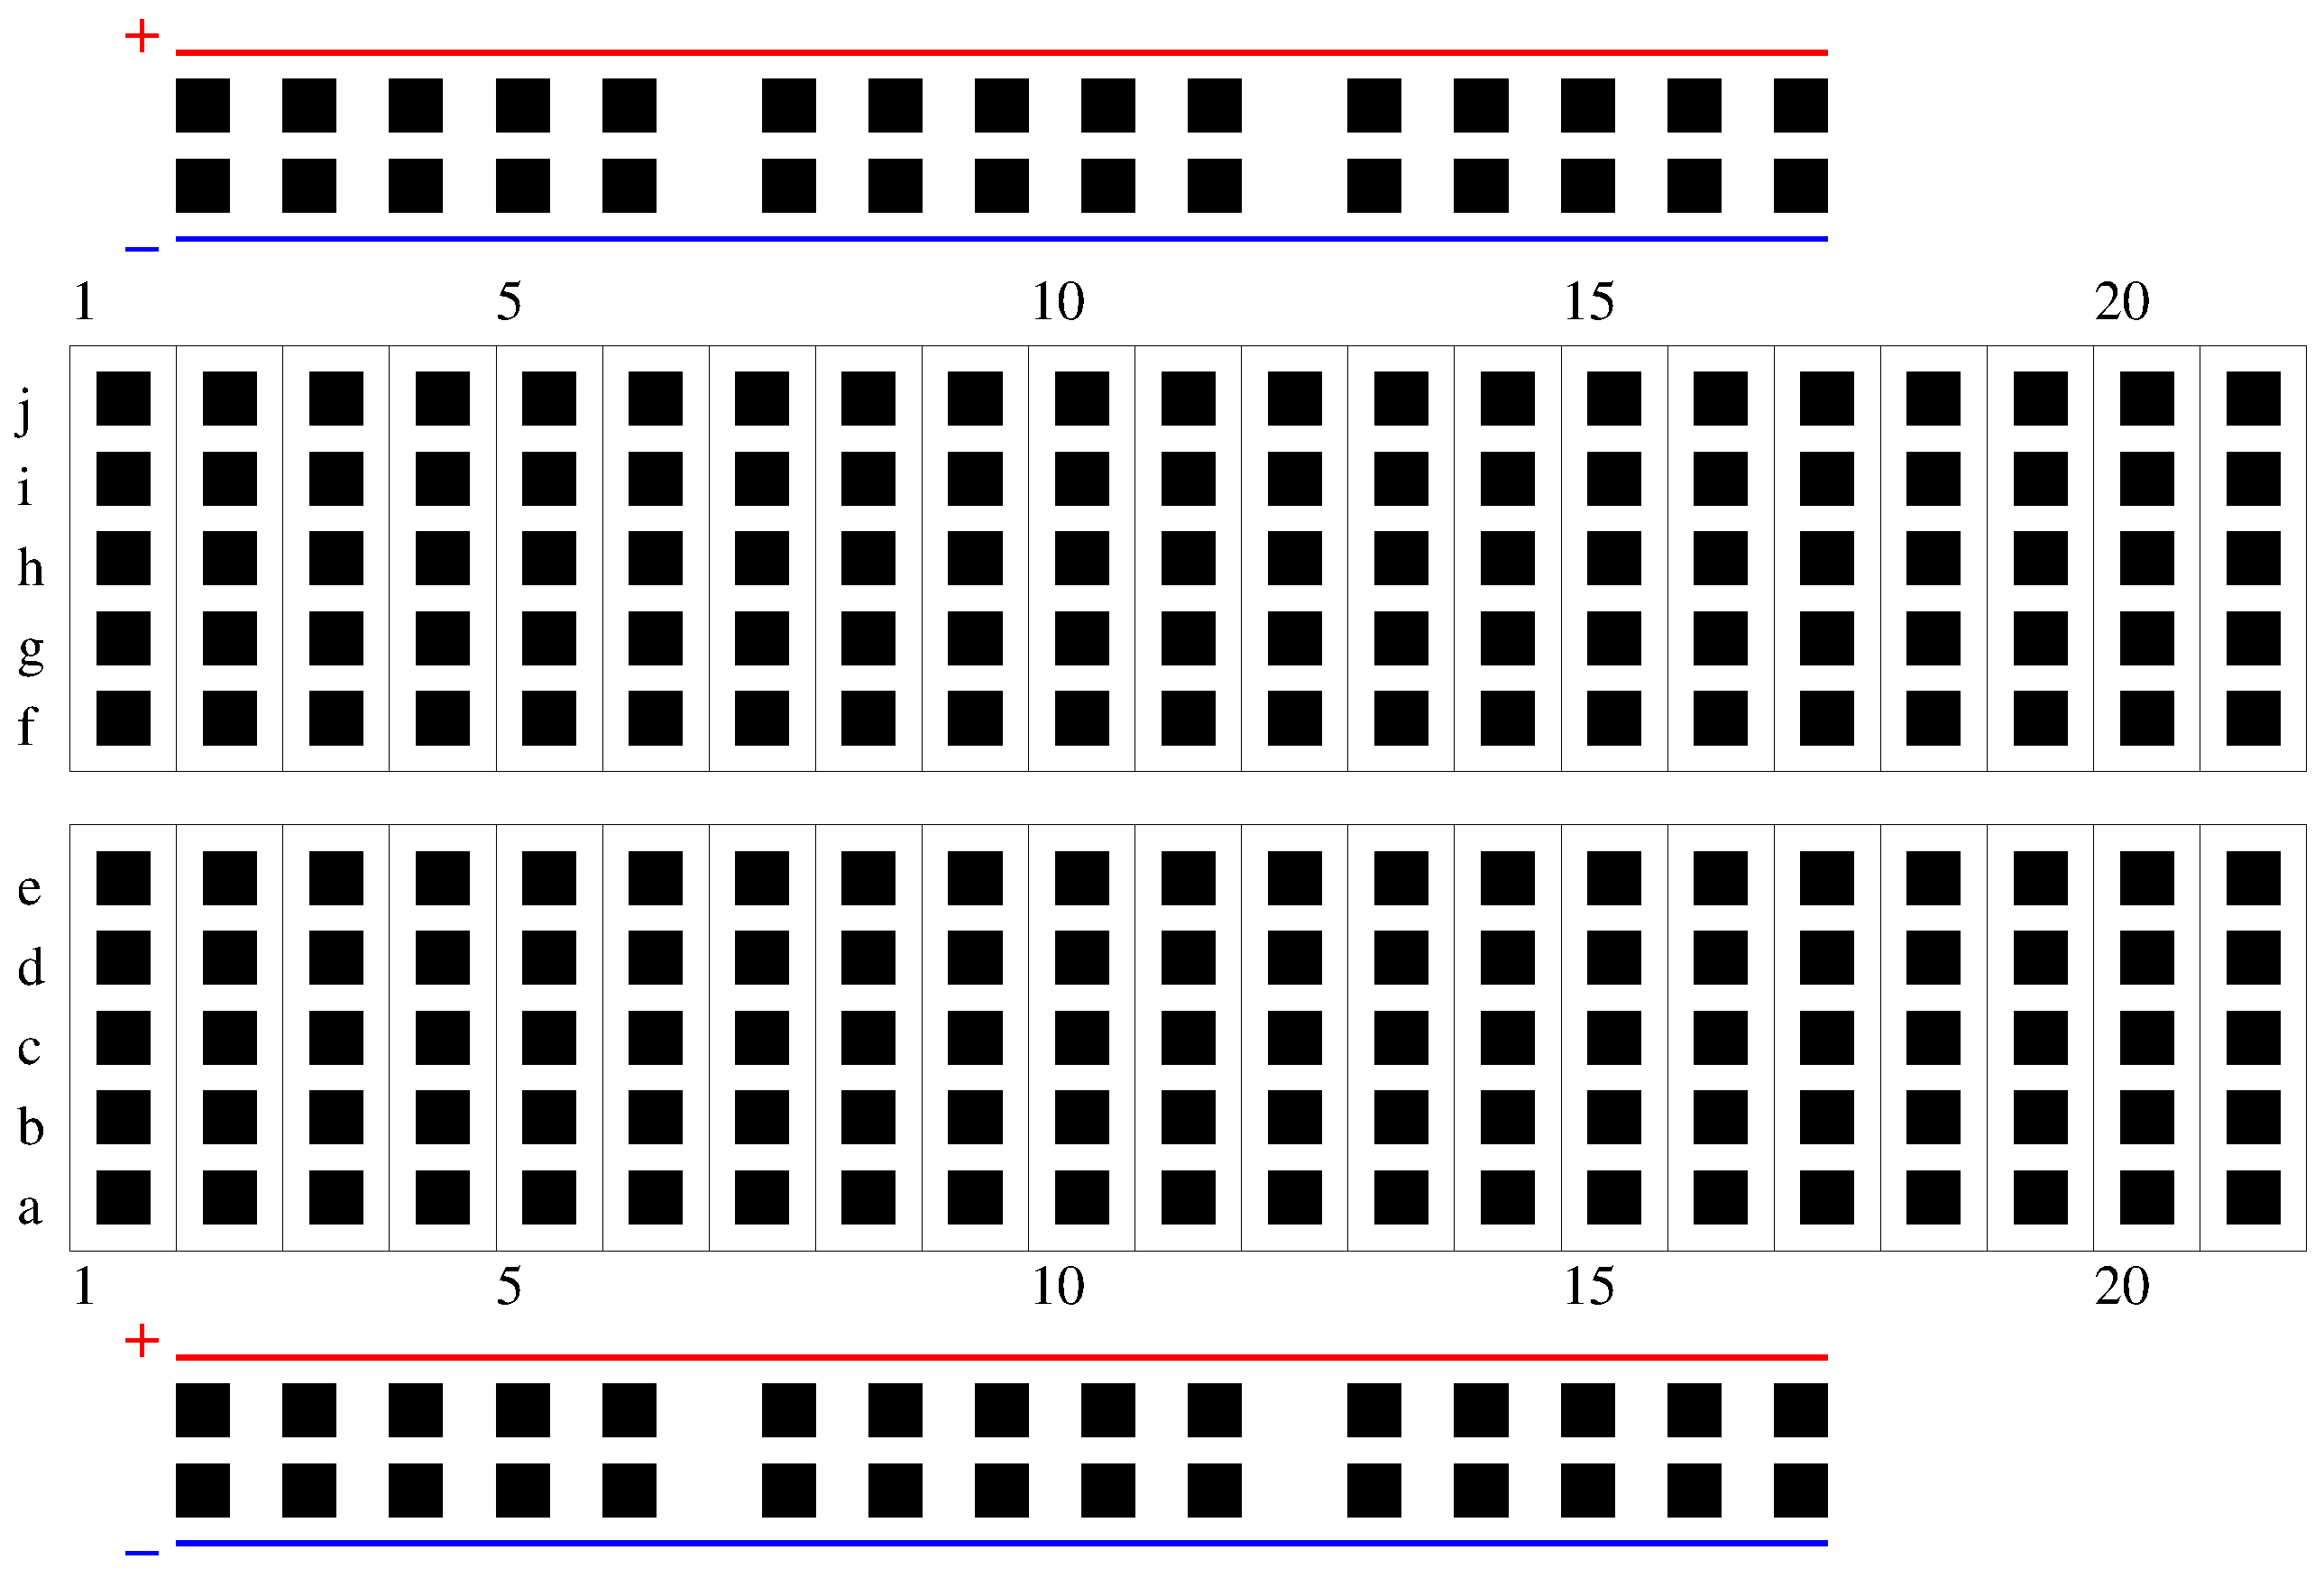
\includegraphics[width=0.7\linewidth]{figures/breadboard.eps}
  \caption{Breadboard
  \label{fig:breadboard}}
\end{figure}

Breadboards will help us to build circuits. It allows for effective connection between components without worrying about the electrical subtleties or hazards. Taking Figure~\ref{fig:breadboard} as a reference, the breadboard has internal electrical connections that makes it possible to tie multiple components to a single point. It does so by representing a \emph{physical} connection as multiple rows of the same column. That is: holes $1$a and $1$d are physically connected inside the breadboard's circuitry, whereas $3$d and $4$a are not.

Each breadboard is divided by thick spaces among different sections. In Figure~\ref{fig:breadboard}, there are four distinct sections: two with the $+$ and $-$ symbols, and two with numbers and letters. The latter was described above, whereas the former works in the opposite way: holes are connected with other holes in the same row. This section is often used to power the circuit, but more on that further in the practice.

Before writing any code, try to assemble the parts as shown in Figure~\ref{fig:blinkingLEDAdvancedLayout}.

\begin{figure}[htbp]
  \centering
  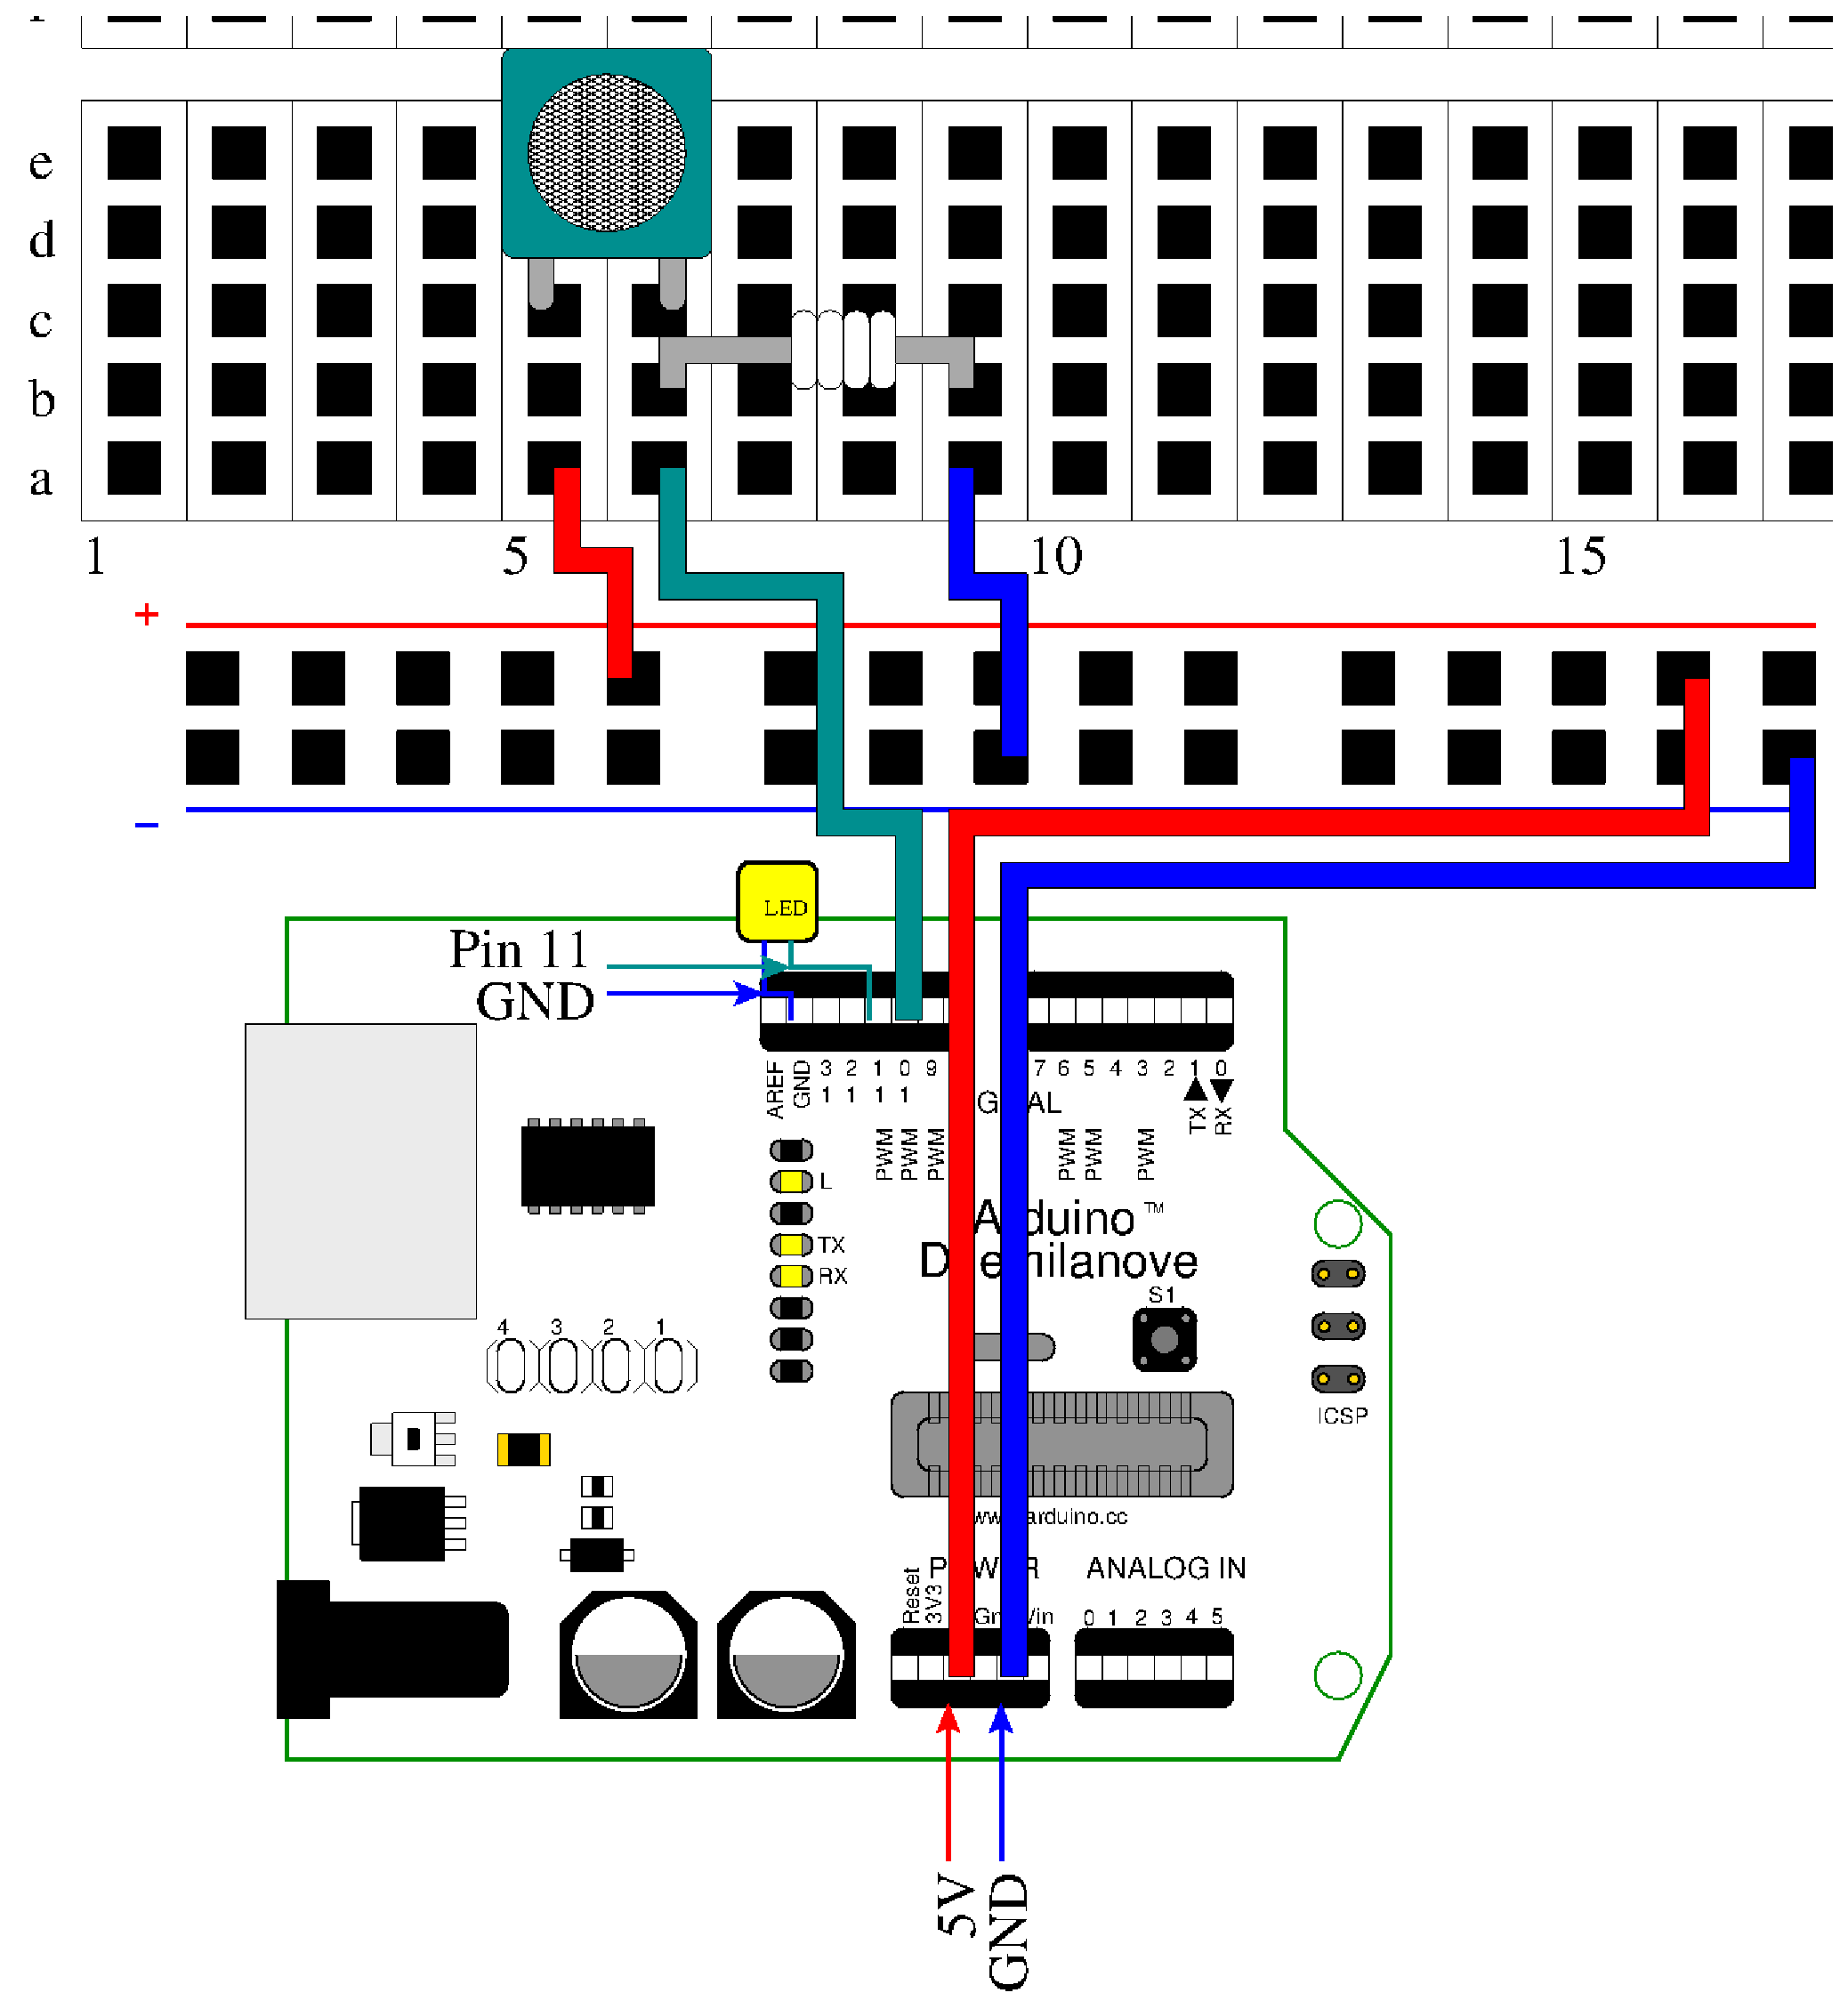
\includegraphics[width=0.7\linewidth]{figures/blinkingLEDAdvanced-scaled.eps}
  \caption{Blinking LED advanced layout
  \label{fig:blinkingLEDAdvancedLayout}}
\end{figure}

To avoid any confusion, let's review the layout component by component:

\begin{enumerate}
	\item Place the pushbutton on your breadboard. In Figure~\ref{fig:blinkingLEDAdvancedLayout}, the two pushbutton "legs" are inserted into holes $5$c and $6$c. In this example, the pushbutton will be energised through the $5$c leg.
	\item Connect one of the legs of the resistor to the negative leg of the pushbutton (hole $6$b). This will physically connect the resistor to one of the legs of the pushbutton. Insert the other leg on hole $9$b.
	\item In order to avoid confusion, cables on all figures are color coded. \emph{Red} represents power cables, \emph{blue} are connections to GND and \emph{cyan} are connections to IO pins on the Arduino.
\end{enumerate}